% \chapter{Conclusões}\label{cap:conclusions}

% As conclusões devem sintetizar e proporcionar uma perspetiva unificadora ao trabalho efetuado. Poderá ser feita uma breve referência a trabalhos de outros com semelhanças ao efetuado e ao conhecimento que resultou do trabalho efetuado, bem como sugestões de trabalho futuro. A coerência do documento implica que as conclusões devem ser coerentes com as ideias expostas na introdução.

\chapter{Características do Sistema do ponto de vista funcional}\label{cap:functions}
%Adicionar capturas de tela e diagramas para exemplificar o uso

Após o detalhamentos dos requisitos, da arquitetura escolhida para o sistema, das tecnologias utilizadas no projeto e do detalhamento da implementação de cada componente do sistema, esse capítulo é voltado para as funcionalidades que compõem a aplicação. O projeto abrange diversas componentes, incluindo uma camada de frontend, uma camada de backend, um módulo de recebimento de dados, um módulo de processamento de dados e o banco de dados, portanto, este capítulo tem como objetivo detalhar o funcionamento de cada funcionalidade do sistema, fornecendo uma visão abrangente de como cada componente interage e contribui para a operação do sistema como um todo.

Cada seção deste capítulo se dedicará a uma funcionalidade específica, examinando seu papel e operação em profundidade, bem como a interação entre diferentes componentes do sistema para sua realização. 


\section[Monitoramento em tempo real]{Monitoramento em tempo real}\label{sec:realtimeMonitoring}

\begin{figure}[htbp]
	\centering
	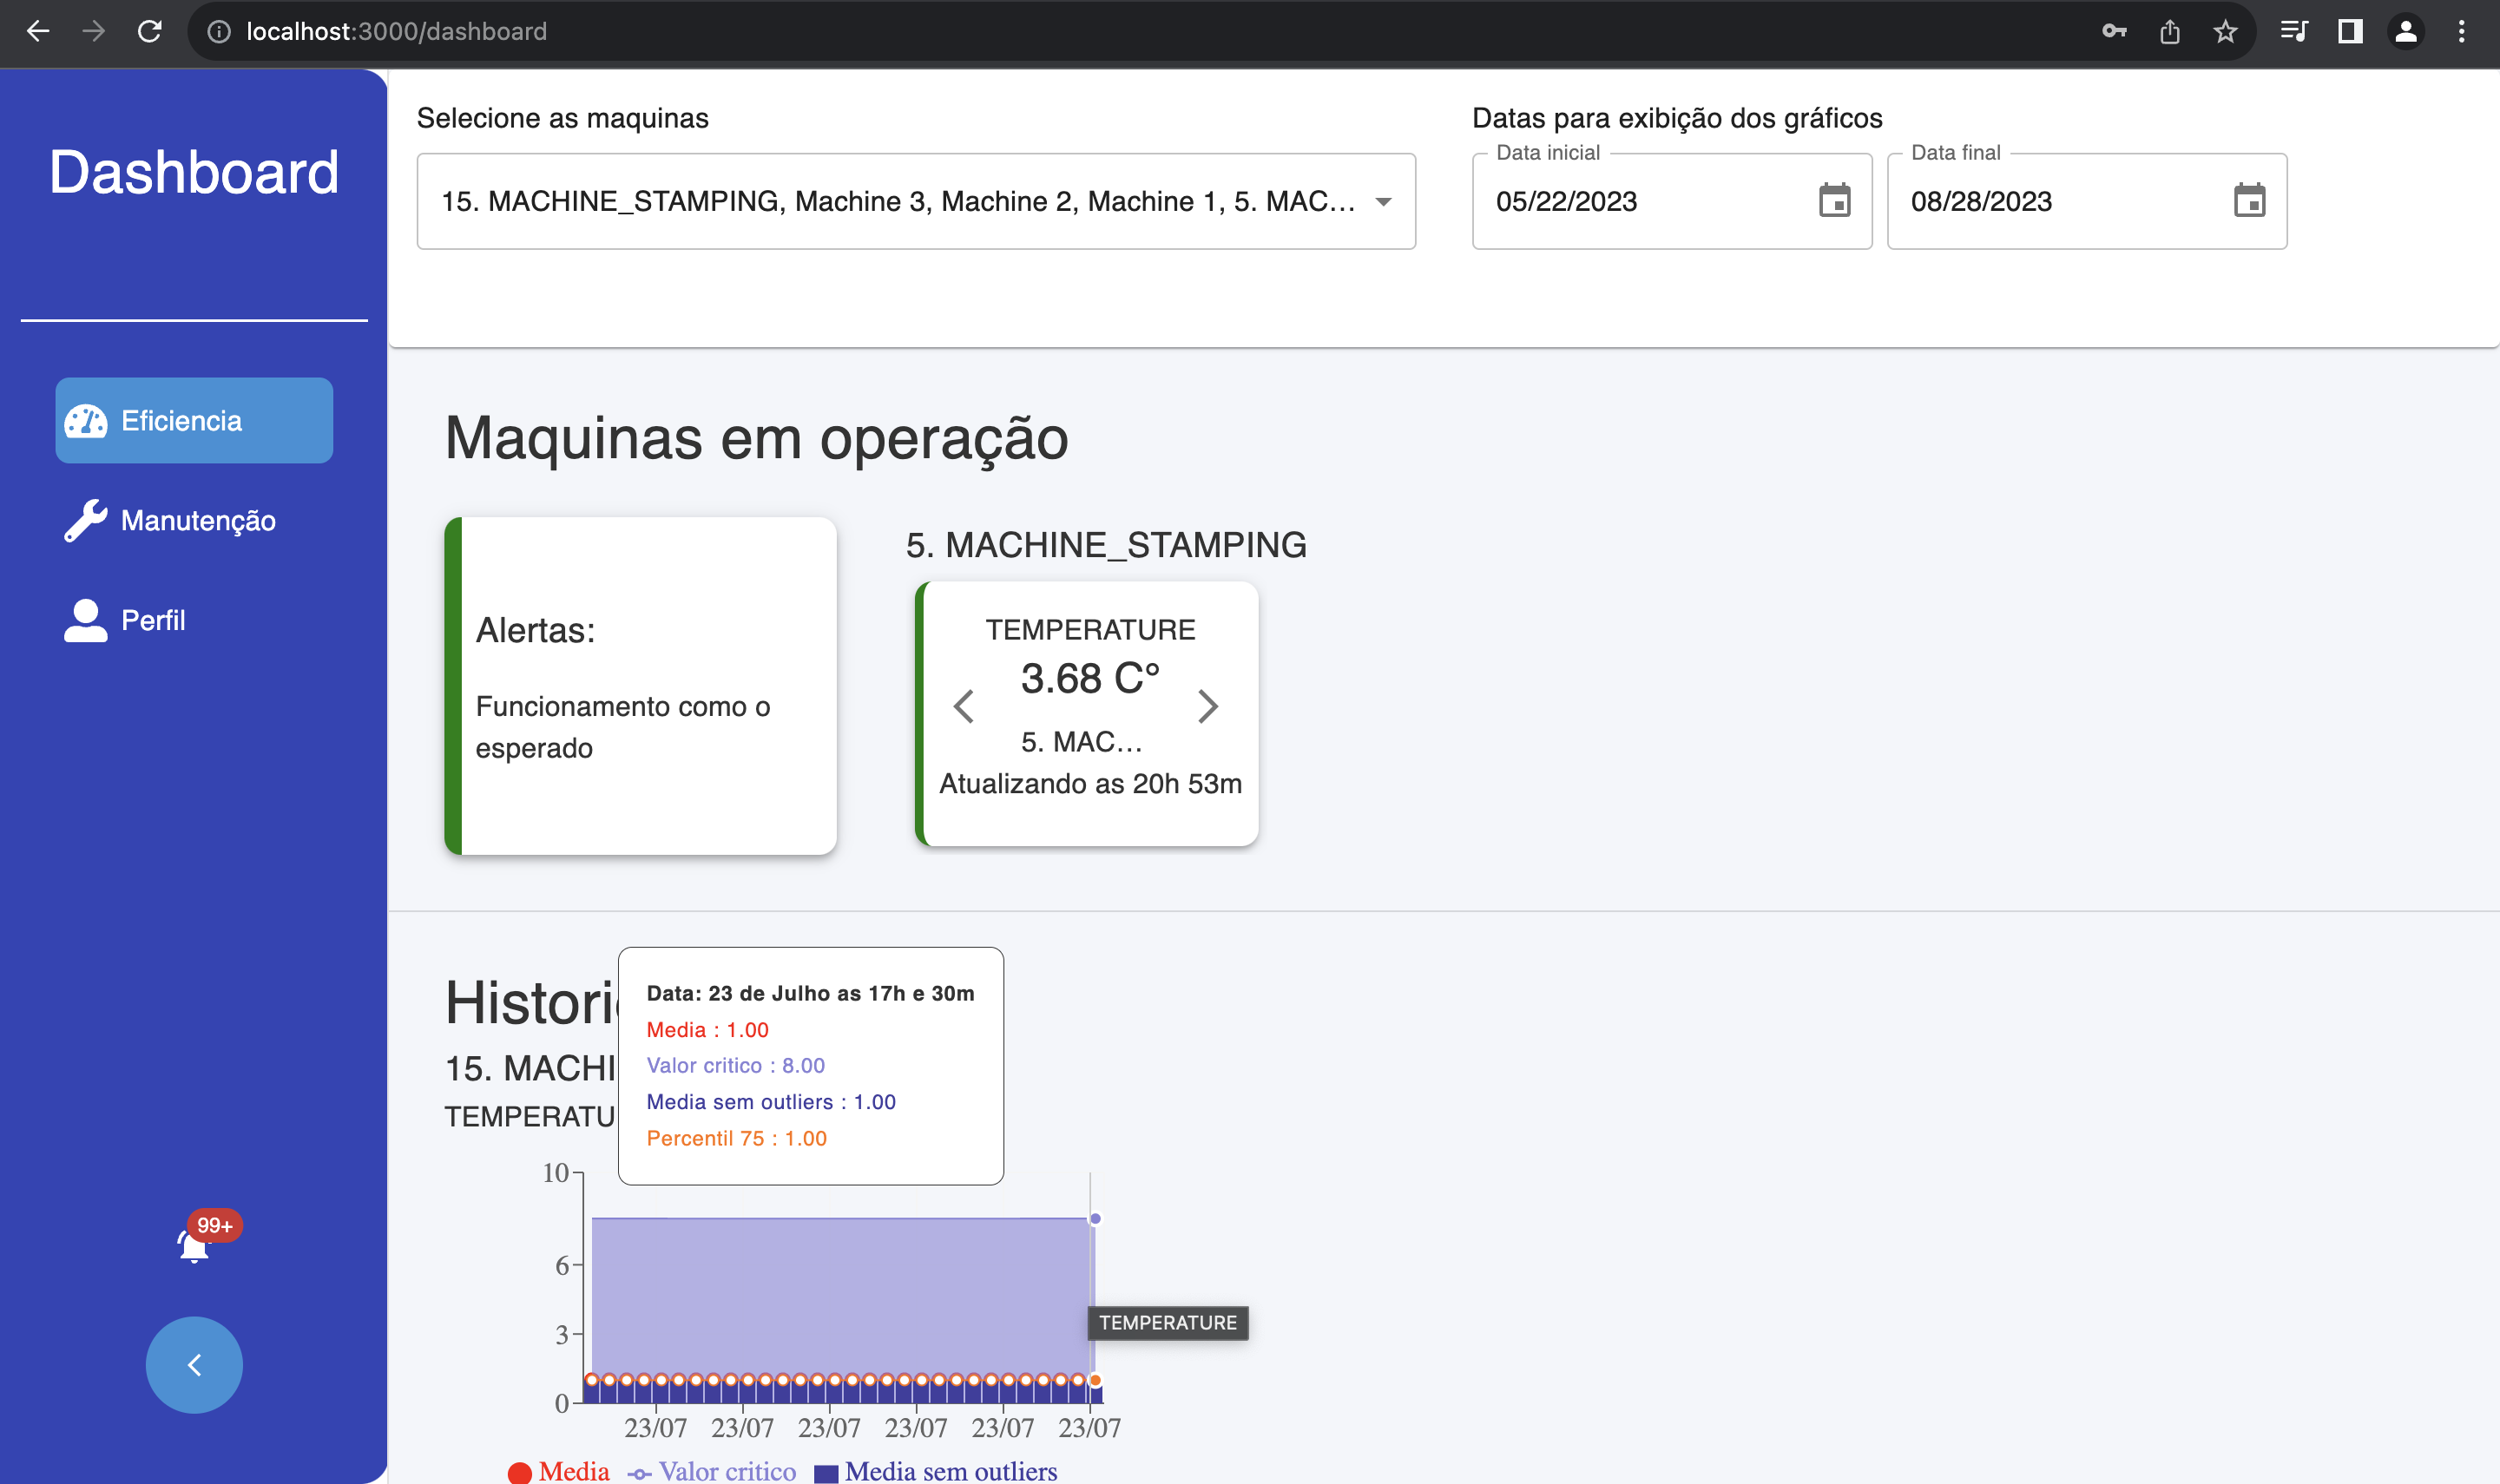
\includegraphics[width=0.7\textwidth]{images/dashboard.png}
	\caption{Dashboard with real time and graph data.}
	\label{fig:dashboradPage}
\end{figure}

No dashboard de interface do usuário são apresentados cartões individuais correspondentes a cada máquina monitorada, na figura \ref{fig:dashboradPage} pode ser visto essa página com um cartão da máquina \texttt{5. MACHINE\_STAMPING}. Em cada cartão, informações dos sensores são exibidas com a possibilidade de navegar entre elas com uma seta direcional. O cartão pode ser visto na figura \ref{fig:cardData}.

\begin{figure}[htbp]
	\centering
	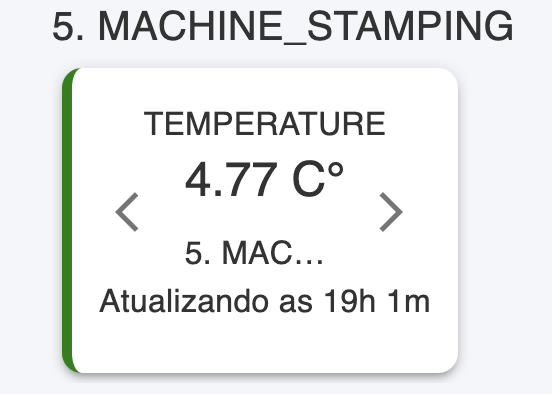
\includegraphics[width=0.4\textwidth]{images/machineCard.png}
	\caption{Card with machine data.}
	\label{fig:cardData}
\end{figure}

%TODO ref para a impl da camada de acesso externo do front
A obtenção desses dados em tempo real é efetuada através de um fluxo contínuo de dados por \textit{streaming}. O frontend da aplicação faz uma requisição ao endpoint \texttt{iot/realtime}, o qual retorna esse fluxo de dados em tempo real. A disponibilização dessa informação ocorre como explicado em X. 

%TODO ref para a impl do modulo de recebimento de dados
Na camada de backend, o fluxo de dados é constantemente alimentado pela classe \texttt{SensorValue}, que por sua vez, é atualizada pelo módulo de recebimento de dados. Ao receber novas leituras dos sensores, o módulo executa validações apropriadas antes de atualizar os valores na classe \texttt{SensorValue}, como explicado em X. Uma vez atualizada, a API acessa esses novos valores e os insere no fluxo de dados transmitido ao usuário conectado.


\section[Alertas e notificações]{Alertas e notificações}\label{sec:alertsAndNotifications}

Esta funcionalidade tem como principal objetivo monitorar o desempenho das máquinas em tempo real e emitir alertas e notificações aos usuários caso sejam detectadas condições de operação inadequadas. Isso permite que ações corretivas sejam tomadas de forma imediata.

%TODO ref para a explicação de metadados
Sempre que uma nova leitura de sensor é recebida pelo módulo de recebimento de dados, uma validação é realizada para verificar se a máquina está operando dentro dos parâmetros aceitáveis. Esses parâmetros são obtidos através dos metadados do sistema, explicado em X.

Se um valor fora do intervalo aceitável é identificado durante a validação, o módulo de recebimento de dados insere uma marcação especial nessa leitura dentro da classe \texttt{SensorValue}. Essa marcação é posteriormente transmitida ao frontend durante o processo de transmissão de dados via \textit{stream}, como explicado em X. %TODO ref para a impl da transmissão em tempo real

Ao receber uma leitura marcada, o frontend atualiza o cartão de informação correspondente para refletir o estado anômalo. Especificamente, dentro do dashboard mostrado na figura \ref{fig:dashboradPage}, a cor do cartão é alterada para vermelho ou amarelo, tanto nos cards individuais, figura \ref{fig:cardData}, quanto no card geral que é usado para mostrar o status geral das maquinas, figura \ref{fig:geralMachineAlert}, portanto, servindo como um alerta visual imediato para o usuário. 

\begin{figure}[htbp]
	\centering
	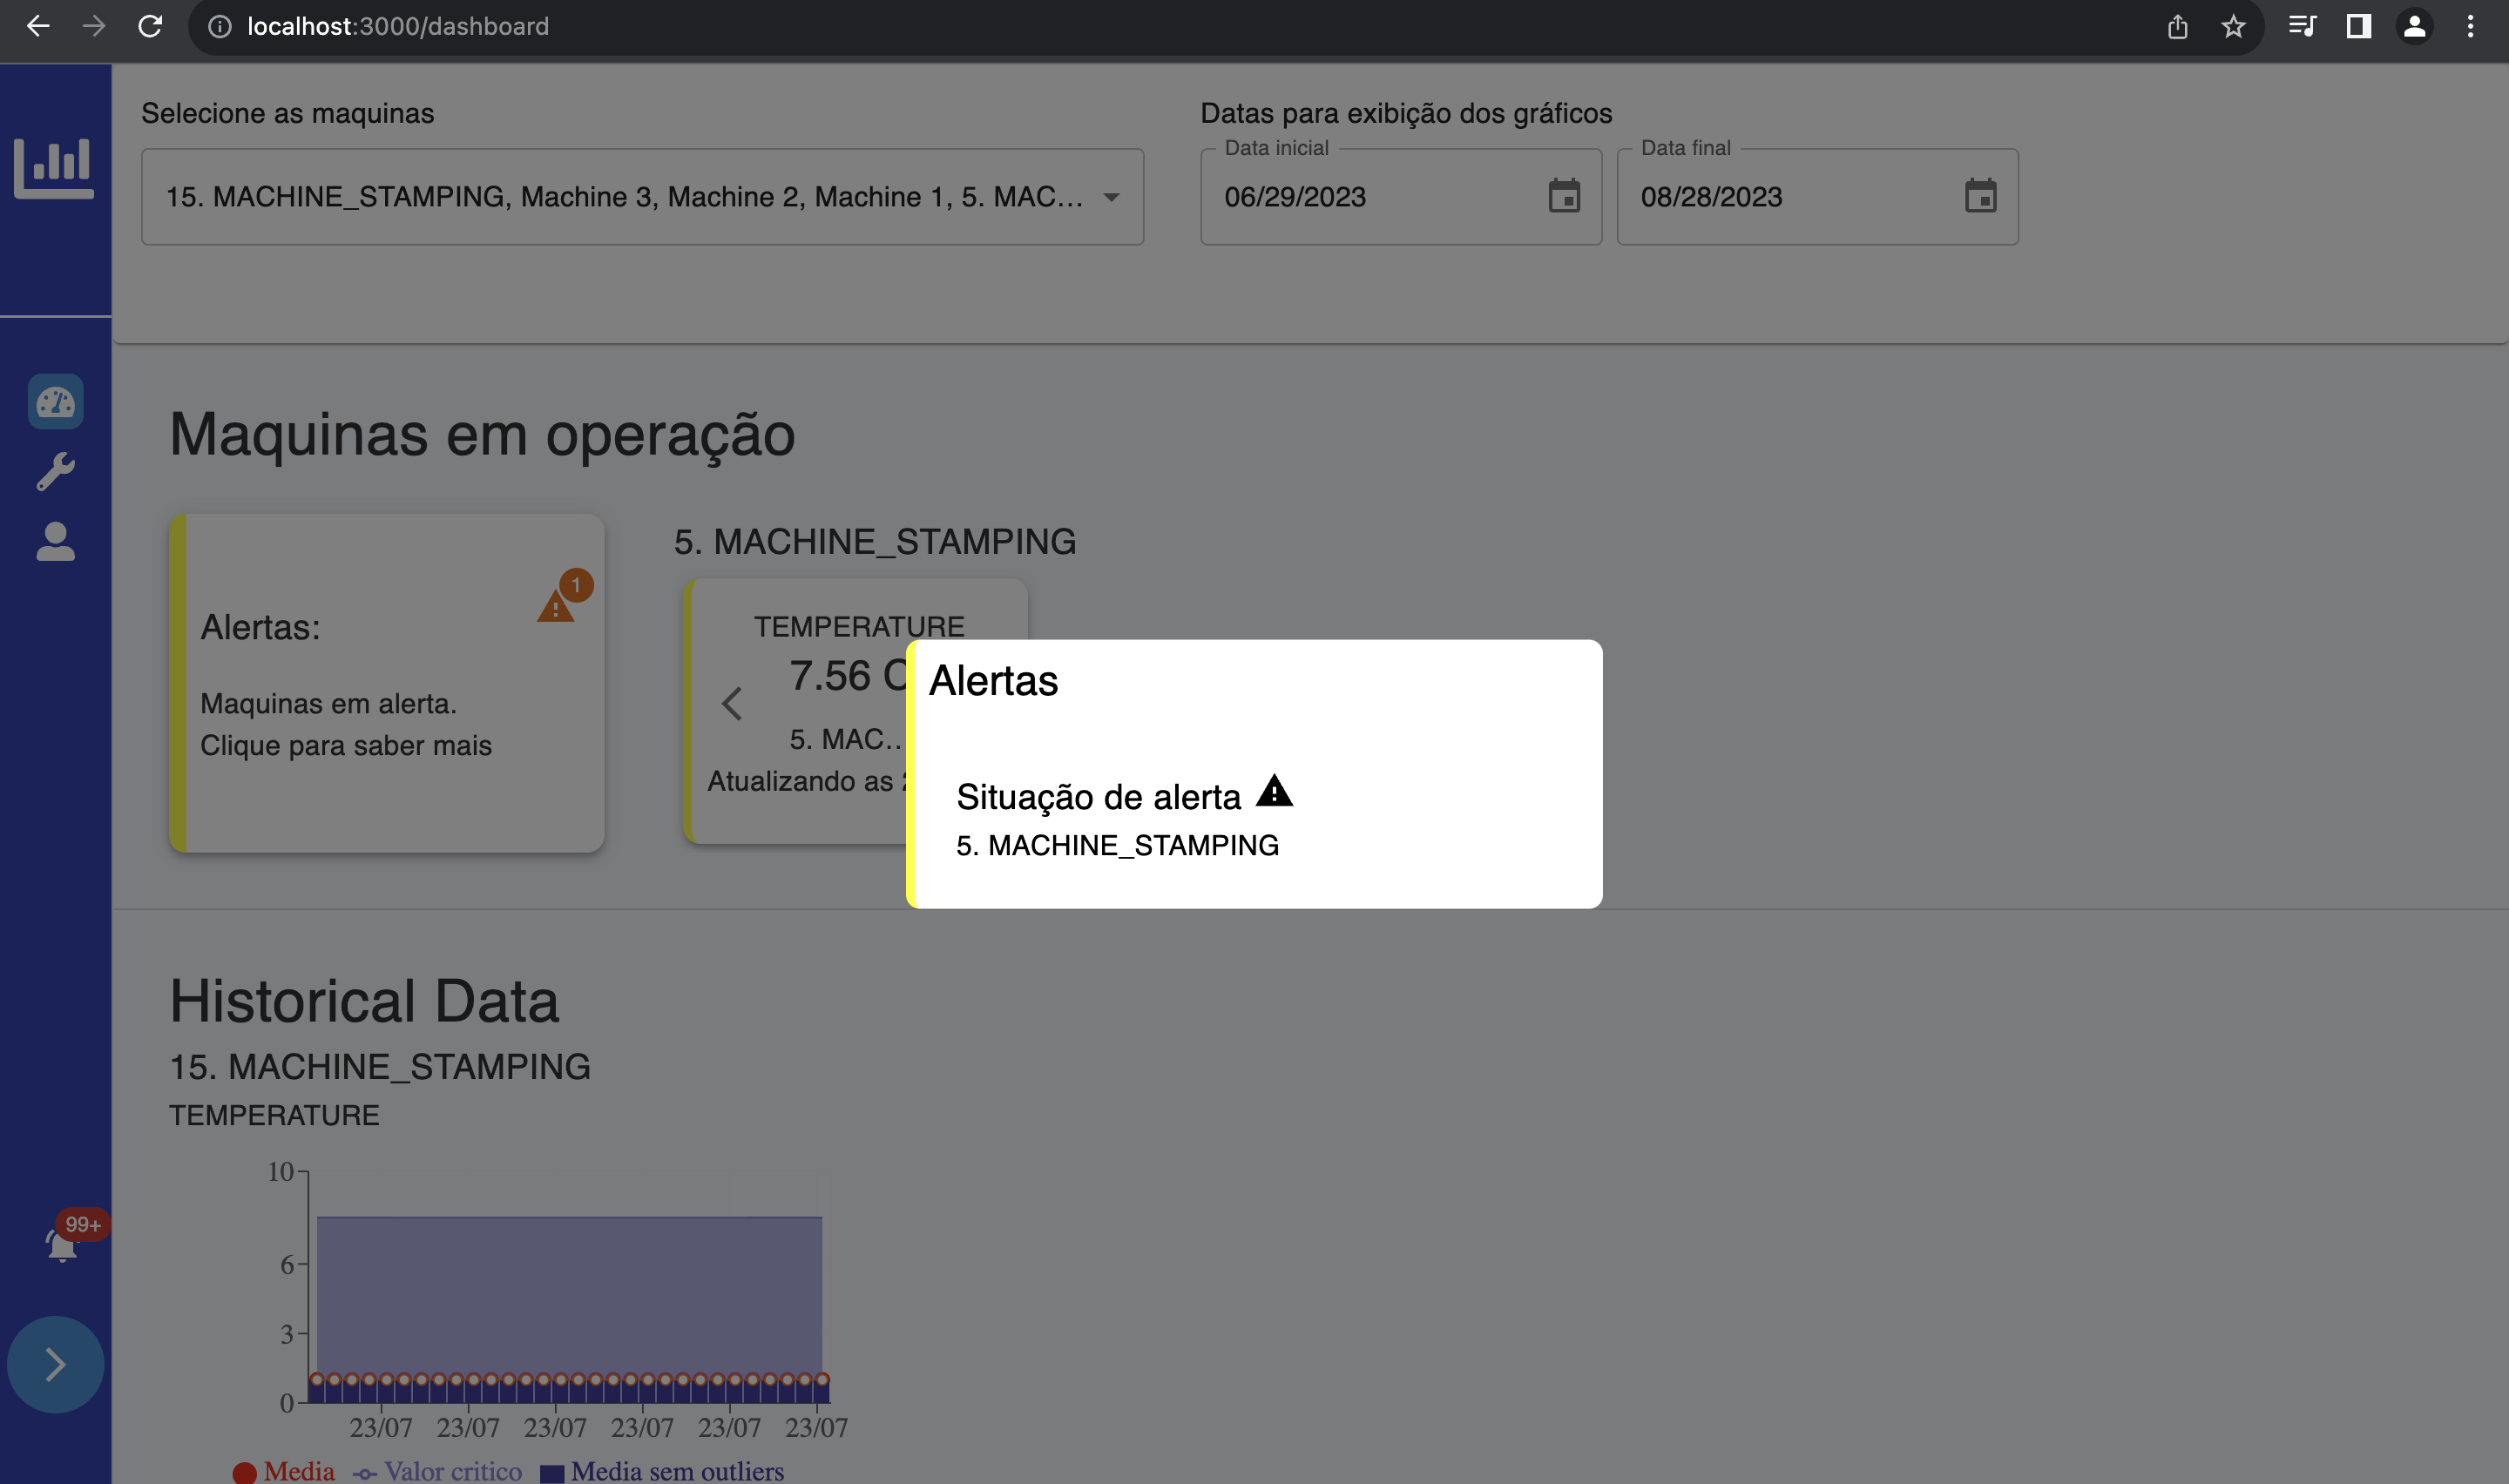
\includegraphics[width=0.8\textwidth]{images/geralMachineAlert.png}
	\caption{General Notifications.}
	\label{fig:geralMachineAlert}
\end{figure}

%TODO ref sub modulo de recebimento de dados que cuida dos alertas
O módulo de recebimento de dados, REF, mantém o controle do estado operacional de cada máquina que está enviando informações. Quando uma máquina sai de um estado de alerta, a ocorrência é registrada no banco de dados, com data de início e término do estado de alerta, junto com as informações referentes ao sensor e à máquina envolvida, como explicado em X. Posteriormente, uma mensagem é enviada aos usuários conectados utilizando a interface de \textit{WebSocket}, informando-os do mau funcionamento da maquina durante o período registrado pelo sistema. %TODO ref impl websocket

As informações sobre a finalização de alertas podem ser acessadas pelos usuários através de notificações na interface do sistema, como pode ser visto na figura \ref{fig:notificationDrawer}. Ao clicar no ícone de notificação no menu lateral do \textit{dashboard}, o usuário pode visualizar essas notificações.

\begin{figure}[htbp]
	\centering
	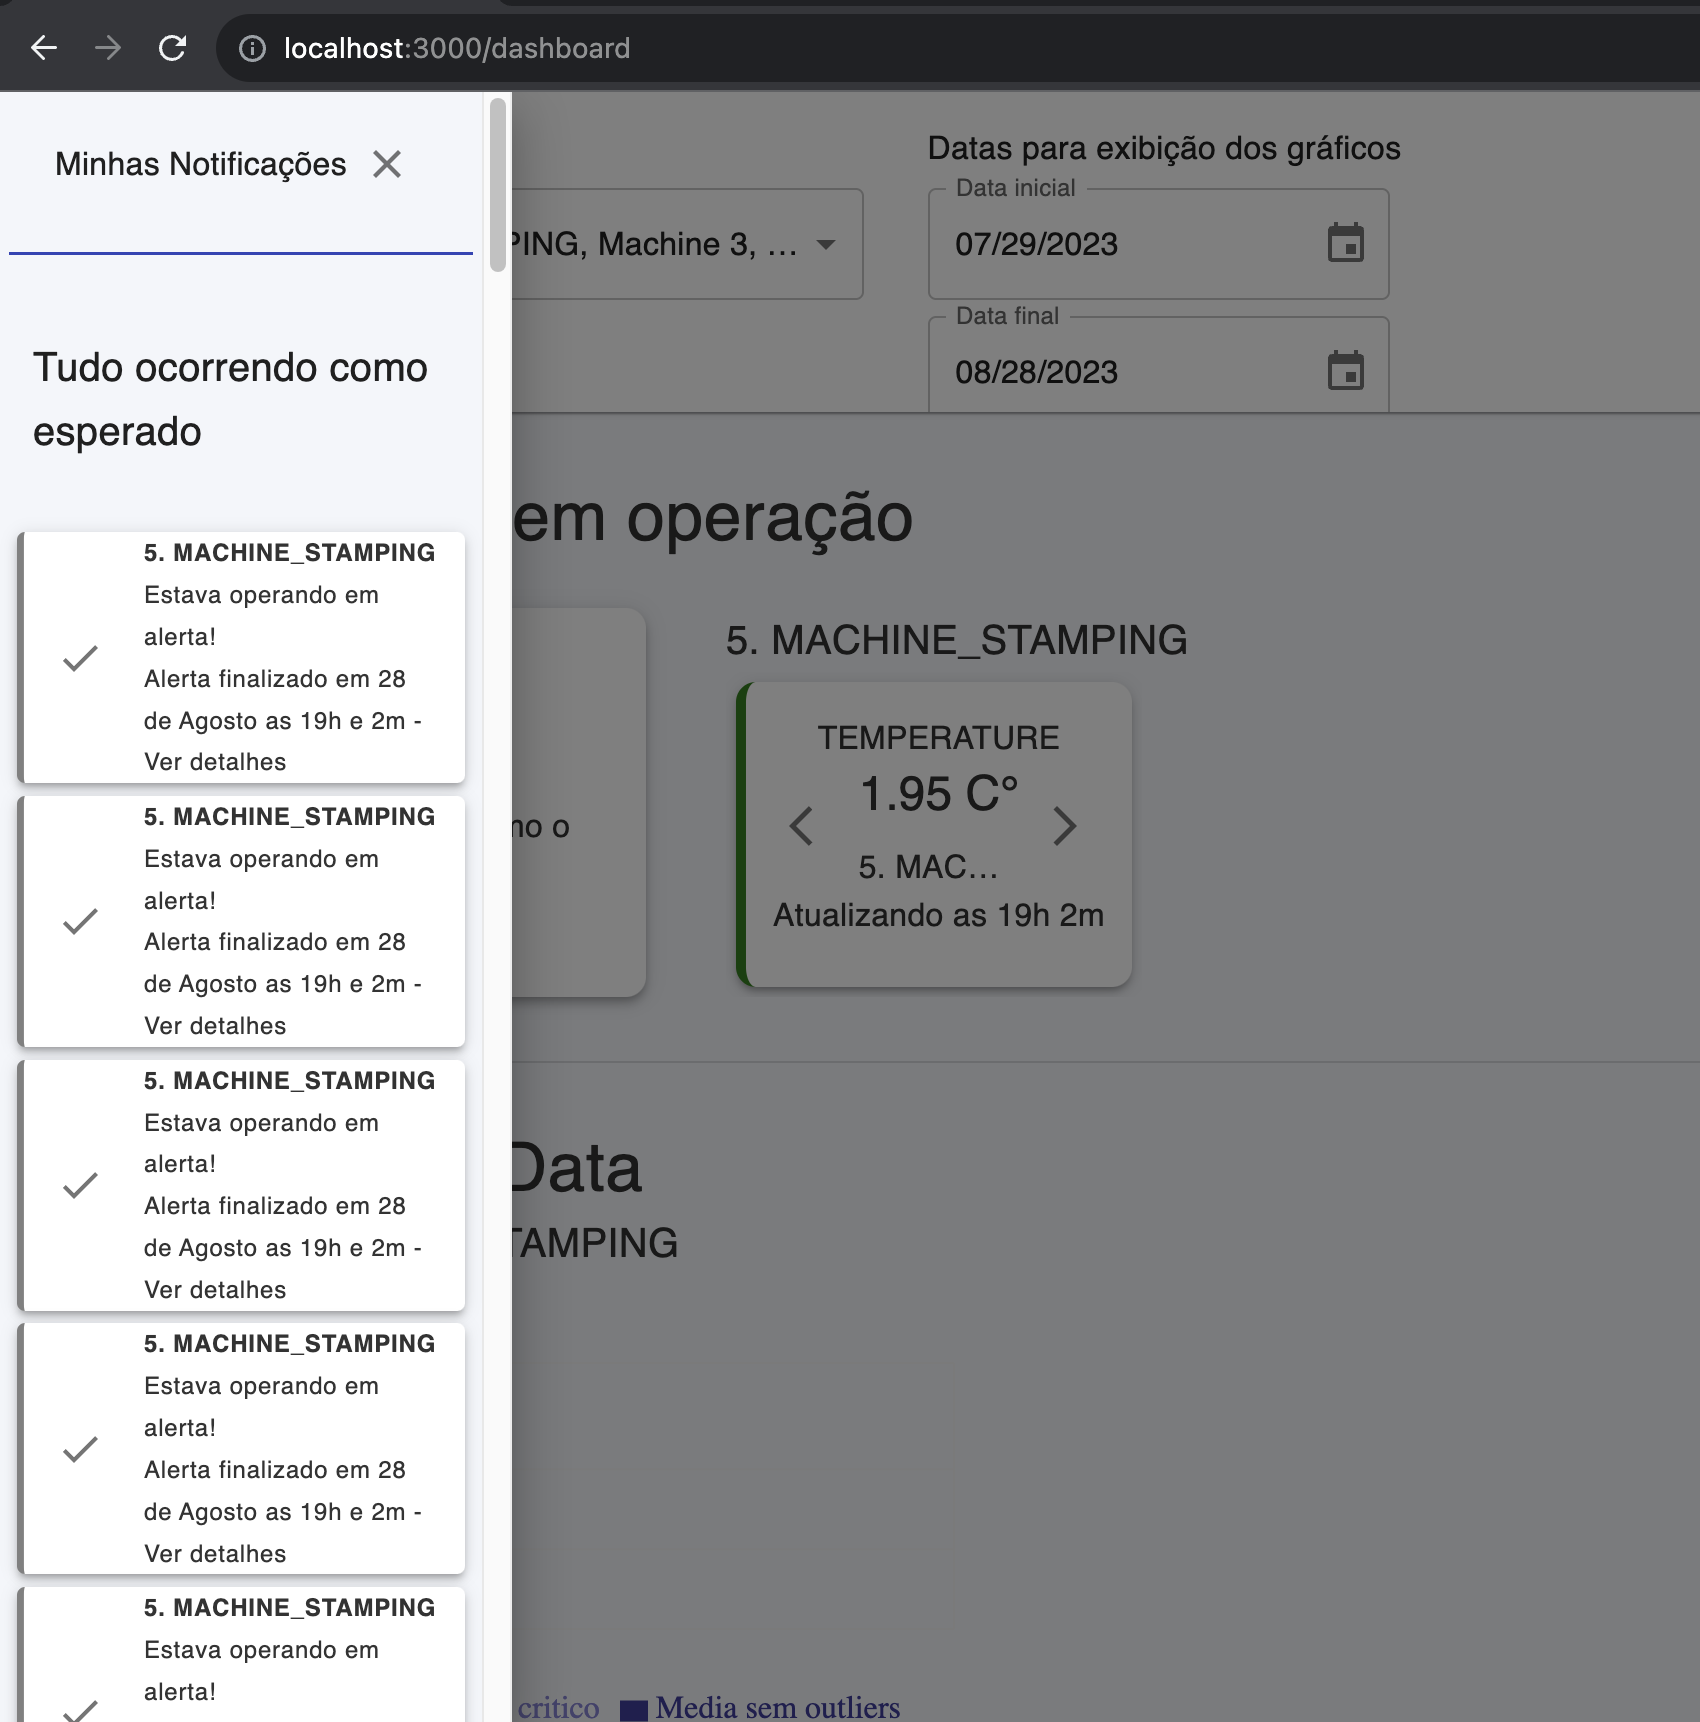
\includegraphics[width=0.6\textwidth]{images/notification.png}
	\caption{Notification drawer.}
	\label{fig:notificationDrawer}
\end{figure}


Portanto, ao iniciar uma sessão no sistema, as notificações anteriores são carregadas para o usuário. Além disso, qualquer nova notificação gerada durante a sessão do usuário é transmitida em tempo real por meio de uma conexão \textit{WebSocket} estabelecida entre o frontend e o backend, como explicado em X.%TODO ref impl websocket


\section[Analise estatística de dados históricos]{Analise estatística de dados históricos}\label{sec:histicalGraphs}

O módulo de processamento de dados é responsável pela análise estatística dos dados históricos. Seguindo o parâmetro padrão do sistema, todos os dias à meia-noite, os dados brutos não processados são lidos e analisados. O resultado da análise é então armazenado no banco de dados para consultas futuras, como explicado em X. %TODO ref modulo de processamento

A possibilidade de acessar esses dados analíticos é providenciada pela API, especificamente pelo módulo "IOT Analytics". A requisição para obter essas informações deve ser autenticada, conforme descrito na seção "Módulos da API".%TODO ref impl API

A representação visual dessas análises é efetuada por meio de gráficos que agregam quatro métricas principais resultantes do processamento. Dessa forma é exibido no gráfico:

\begin{itemize}
    \item \textit{Valor Ideal}: Representado em um gráfico de área, serve como um parâmetro de funcionamento ideal para fornecer uma perspectiva relativa aos outros dados.
    \item \textit{Percentil 75}: Exibido em um gráfico de linha, esta métrica oferece uma visão sobre a distribuição dos valores durante o período de agregação e sua evolução ao longo do tempo.
    \item \textit{Média da Agregação}: Representada em um gráfico de dispersão, esta métrica fornece o valor médio dos dados agregados.
    \item \textit{Média com Remoção de \textit{Outliers}}: Ilustrada em um gráfico de barras, esta métrica é calculada após a remoção dos valores \textit{outliers}, conforme determinado pelo método de construção do boxplot.
\end{itemize}

Portanto, a imagem \ref{fig:graphData} mostra como fica a visualização dessas informações dentro do dashboard.

\begin{figure}[htbp]
	\centering
	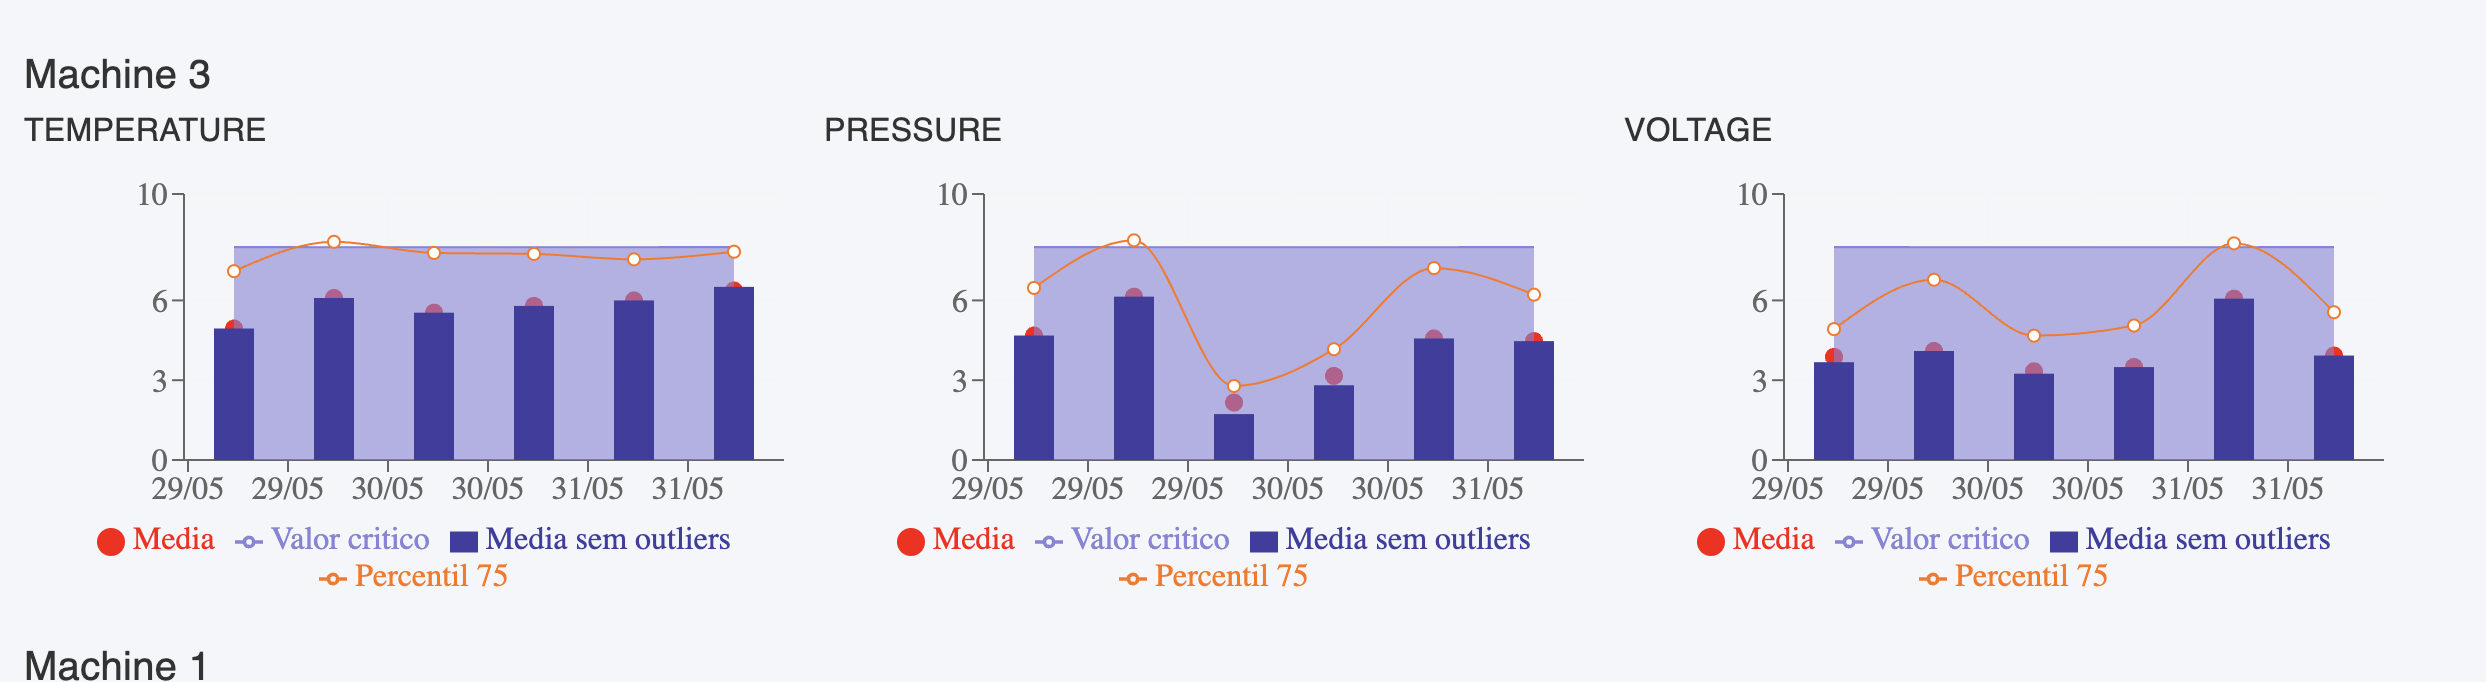
\includegraphics[width=0.7\textwidth]{images/graphData.png}
	\caption{Graph example.}
	\label{fig:graphData}
\end{figure}

\section[Exibição dos dados referente a paragem das máquinas]{Exibição dos dados referente a paragem das máquinas}\label{sec:downtime}

%TODO ref para a parte que explica melhor sobre isso XX
Esta funcionalidade é dedicada à exibição de dados relacionados às paragens das máquinas, armazenados previamente no banco de dados. Como esclarecido na seção XX, a funcionalidade tem o objetivo de demonstrar como seriam apresentados esses dados, caso fossem recebidos pelo sistema de forma similar aos dados dos sensores. A fonte dos dados para a elaboração desses gráficos provém de três planilhas recebidas no início do desenvolvimento do projeto, em que as informações foram salvas no banco de dados. Esses dados são acessados pelo frontend por meio do módulo \texttt{downtime\_analytics} da API.

Os gráficos gerados para representar esses dados são apresentados na forma de gráficos de coluna. Cada gráfico exibe um título correspondente à planilha da qual os dados foram extraídos. A legenda do gráfico indica a porcentagem que cada parada específica representa em relação ao total de paragens.

Os gráficos de coluna fornecem uma maneira eficaz de comparar as diferentes paragens das máquinas, como pode ser visto na figura \ref{fig:downtime}. Esta visualização oferece um meio para analisar a eficiência operacional, identificar possíveis áreas para melhoria e acompanhar o resultado das ações tomadas em relação a paragem das máquinas e a manutenção preditiva.

\begin{figure}[htbp]
	\centering
	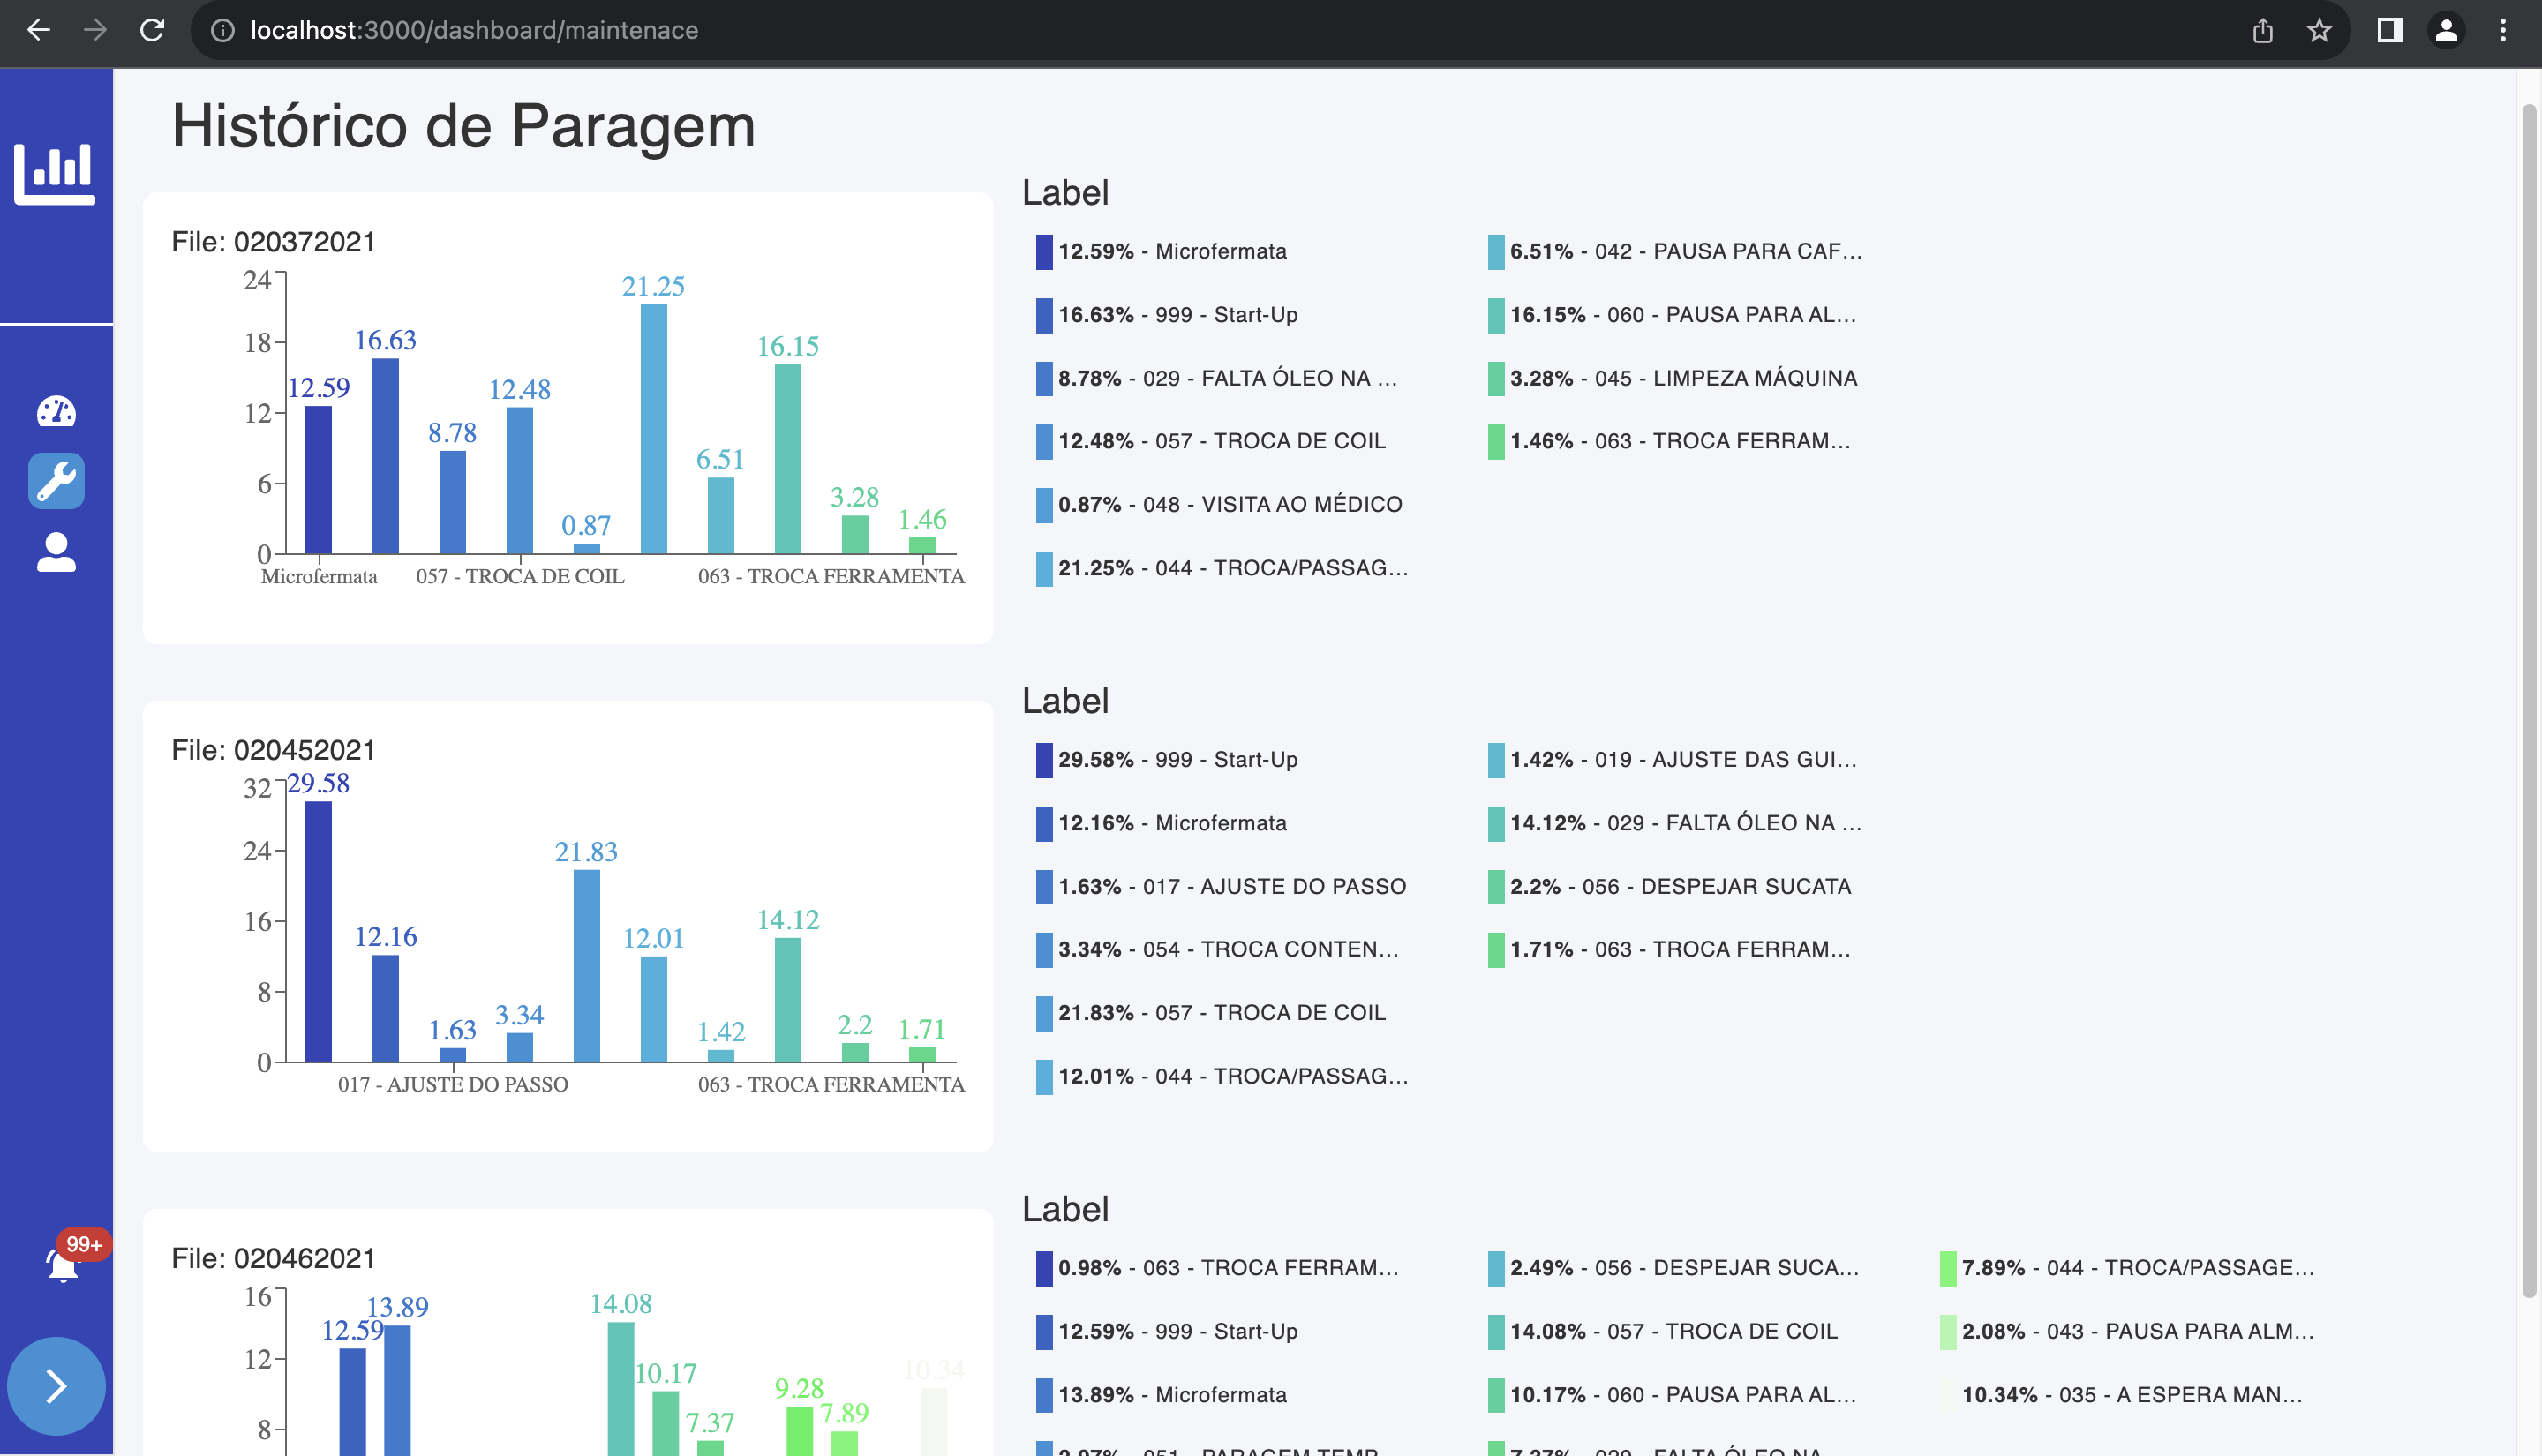
\includegraphics[width=0.75\textwidth]{images/downtime.png}
	\caption{Downtime graph.}
	\label{fig:downtime}
\end{figure}

\section[Perfil de usuário]{Perfil de usuário}\label{sec:profile}

A funcionalidade de perfil de usuário foi desenvolvida com o objetivo de fornecer aos usuários acesso aos seus dados pessoais armazenados no sistema. Além da visualização dessas informações, esta tela permite também a realização de modificações, incluindo a alteração de senha, e-mail e outros dados pessoais como nome, sobrenome e descrição.

%TODO ref para a parte de modulos da API
Para ler e modificar os dados apresentados, o módulo \textit{User} da API é utilizado REF. Este módulo disponibiliza endpoints que permitem o acesso e a modificação dos dados armazenados, garantindo que as informações sejam atualizadas conforme as interações do usuário, como pode ser visto na figura \ref{fig:profilePage}.

Um recurso adicional fornecido por esta tela é a opção de logout. Ao selecionar esta opção, todas as informações armazenadas do lado do cliente são apagadas, efetuando assim a saída segura do usuário do sistema.

\begin{figure}[htbp]
	\centering
	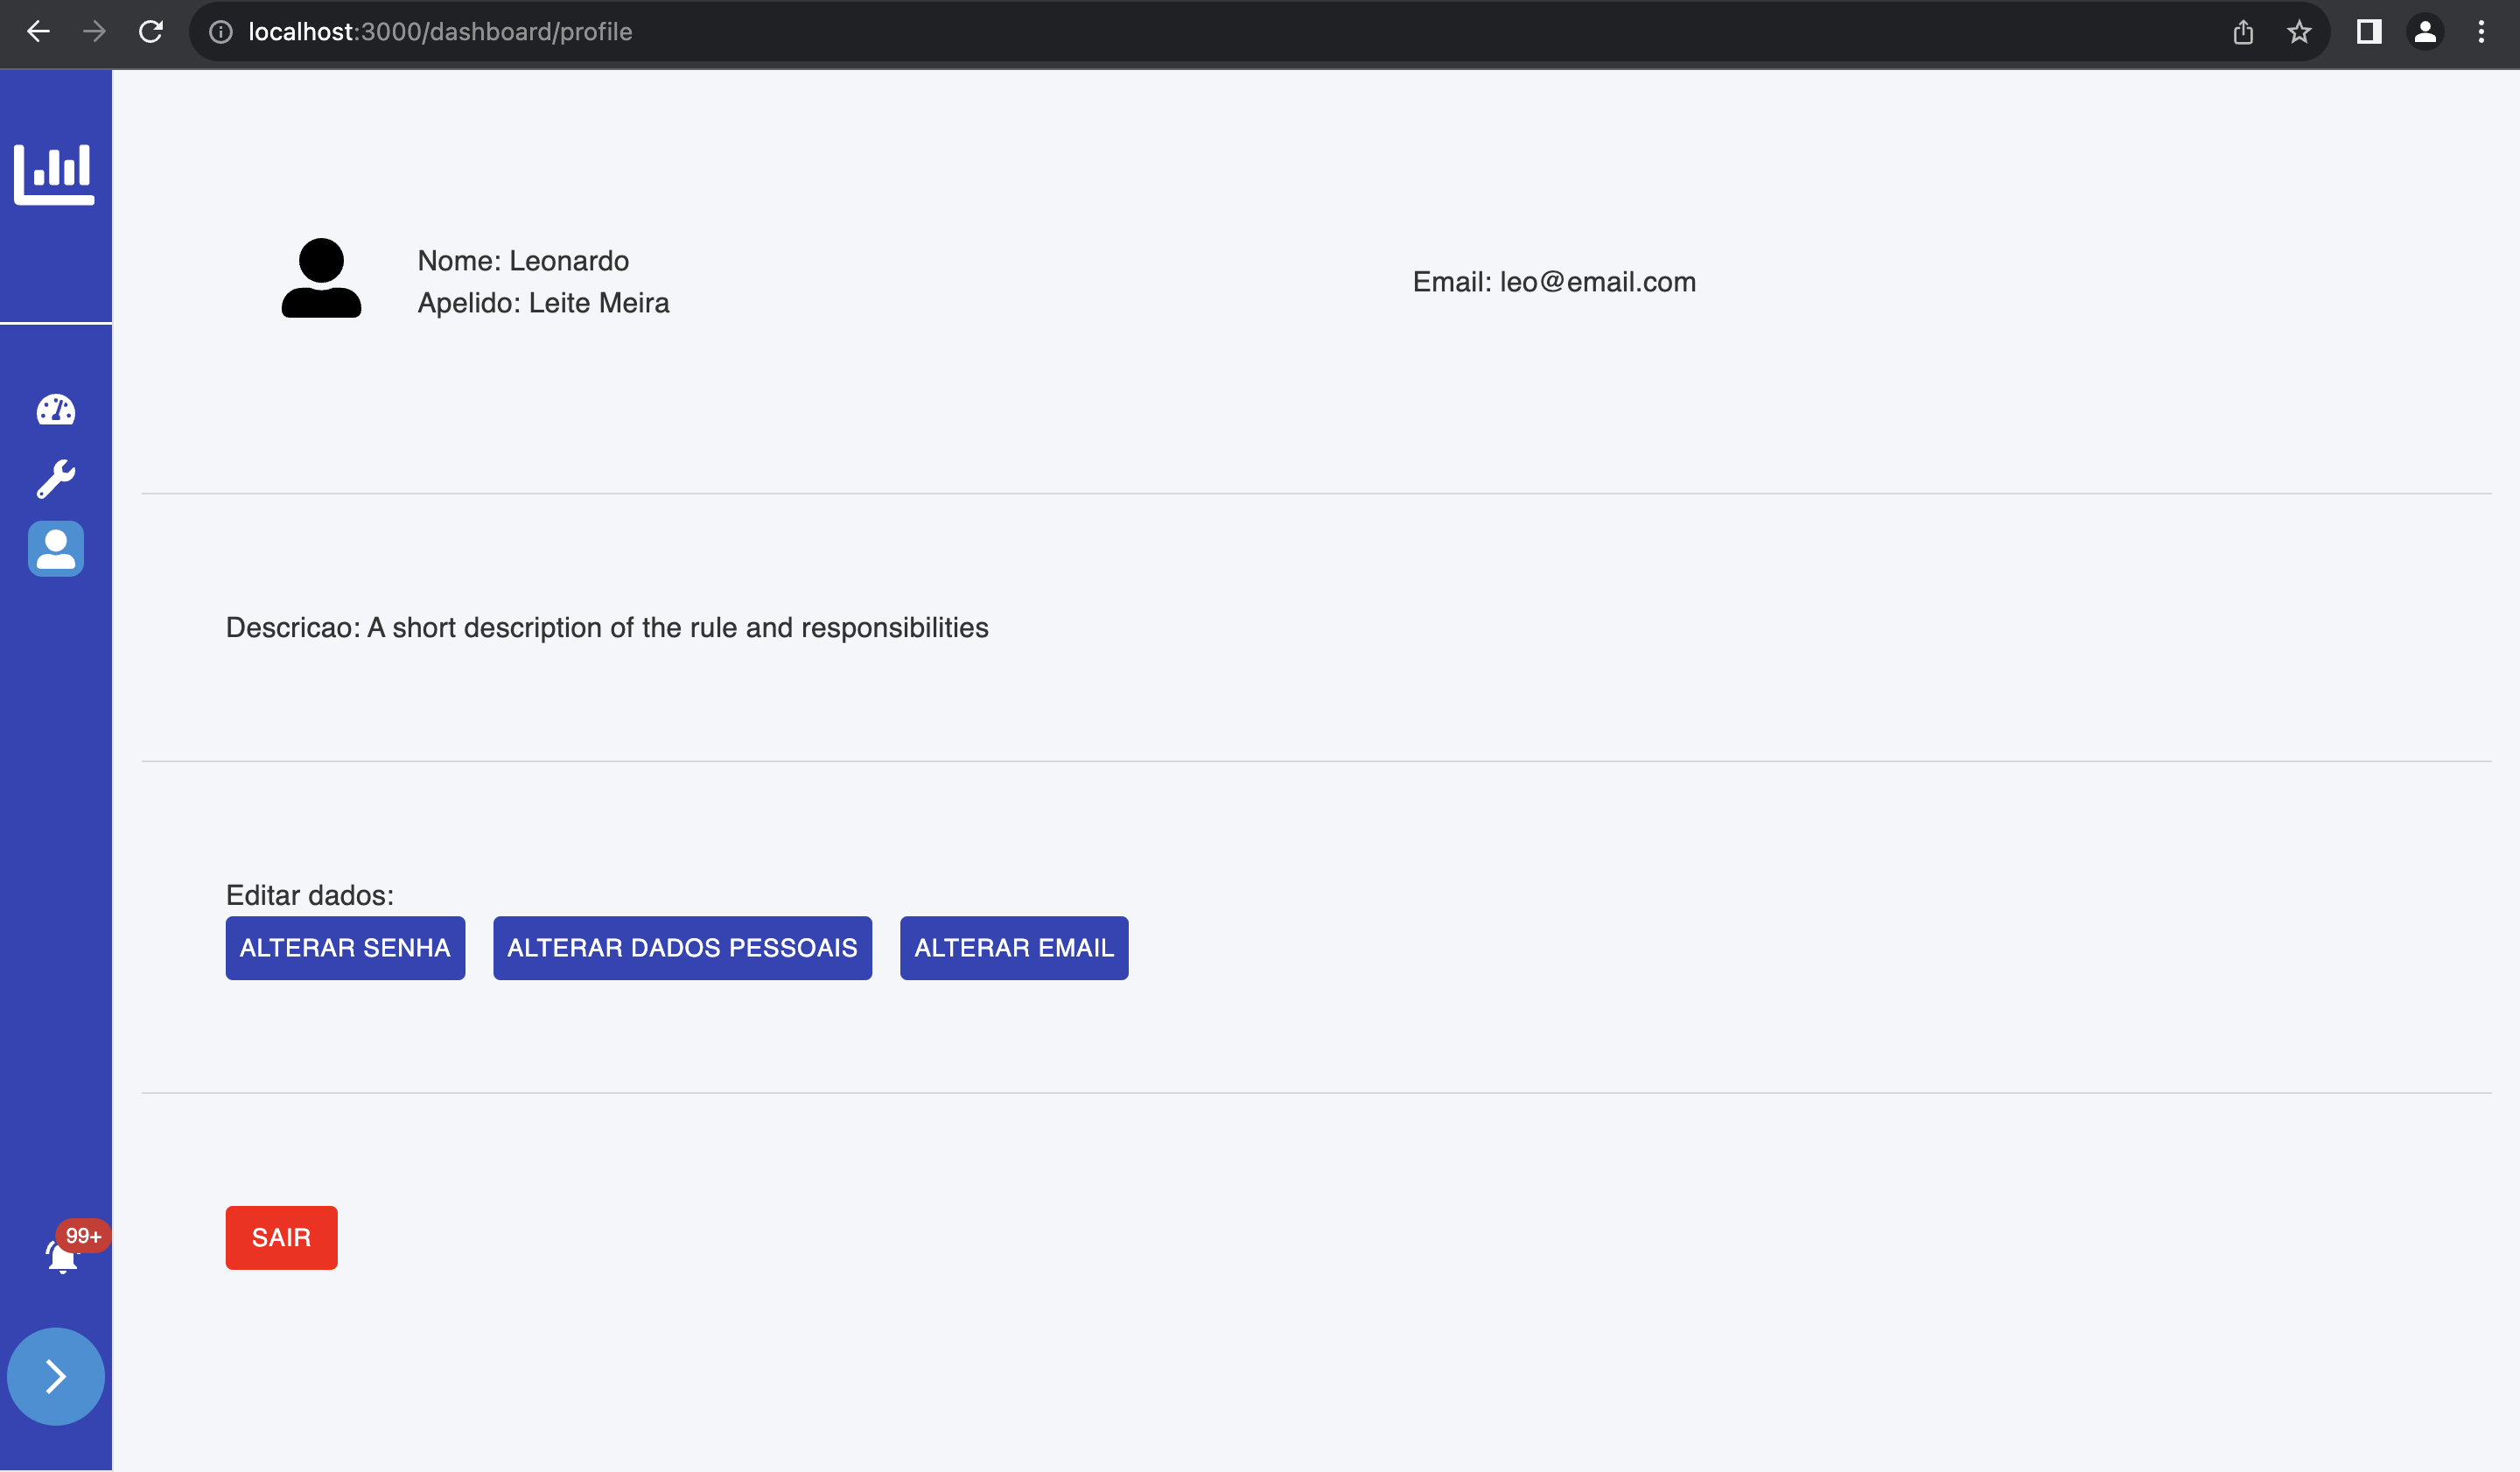
\includegraphics[width=0.8\textwidth]{images/profile.png}
	\caption{Profile page.}
	\label{fig:profilePage}
\end{figure}

